\documentclass[10pt]{book}

\usepackage[T1]{fontenc}
\usepackage{kpfonts}
\usepackage{amsmath}
\usepackage{amssymb}
\usepackage{amsthm}
\usepackage{mathtools}
\usepackage{empheq}
\usepackage{pgfplots}
\usepackage{cleveref}
\usepackage{graphicx}
\usepackage{geometry}
\usepackage{titlesec}
\usepackage{fancyhdr}
\usepackage{setspace}
\usepackage{microtype}
\usepackage{parskip}
\usepackage{tcolorbox}
\usepackage{booktabs}
\usepackage{float}

\geometry{a5paper, top=1.5cm, bottom=2cm, inner=1.8cm, outer=1.2cm}

\titleformat{\chapter}[display]{\normalfont\large\bfseries}{\chaptertitlename\ \thechapter}{10pt}{\large}
\titleformat{\section}{\normalfont\normalsize\bfseries}{\thesection}{1em}{}
\titleformat{\subsection}{\normalfont\small\bfseries}{\thesubsection}{1em}{}

\pgfplotsset{compat=1.18}

\title{Mathematical Analysis}
\author{London Wallace}
\date{Semester 1, 2026}

\renewcommand{\chaptermark}[1]{\markboth{#1}{}}

\pagestyle{fancy}
\fancyhf{}
\fancyfoot[C]{\thepage}
\renewcommand{\headrulewidth}{0pt}
\fancypagestyle{plain}{\fancyhf{}\fancyfoot[C]{\thepage}\renewcommand{\headrulewidth}{0pt}}

\fancypagestyle{plain}{\fancyhf{}\renewcommand{\headrulewidth}{0pt}}

\setstretch{1.15}

\titlespacing{\chapter}{0pt}{-10pt}{10pt}

\newcommand{\newthought}[1]{\vspace{0.5\baselineskip}\noindent{\scshape #1}}

\renewcommand{\bibname}{Bibliography and Suggested Reading}

\begin{document}
\frontmatter
\maketitle
\tableofcontents

\chapter{Preface}
\newthought{These notes} are based primarily on Michael Spivak's \emph{Calculus}, and Stephen Abbott's
\emph{Understanding Analysis}, with intermittent input from Terence Tao's fantastic, \emph{Analysis I}. The main focus
has been on presenting solutions and problem-solving techniques for as many problems as possible, prefaced with only as
concise an introduction as necessary to understand their motivation.

\section{What is Analysis?}

\newthought{Real Analysis} is the rigorous study of real numbers, sequences and series of real numbers, and functions of real
numbers. It seeks to precisely understand the behaviour of these objects and is the theoretical foundation for the field
of Calculus, which is the study of change. It is related to, but distinct from, \emph{complex analysis} which is the study
of complex numbers and their functions, \emph{harmonic analysis} which is the study of waves like sine and cosine, and how
they synthesize other functions via the Fourier transform, and \emph{functional analysis} which concentrates more on functions
and how they form things like vector spaces and so forth. \cite{tao-analysis}.

\newthought{This text} will focus only on \emph{real} analysis. Specifically, we want to know
\begin{enumerate}
  \item What is a function? What does it mean for a function to have a limit? to be continuous? bounded? How do these
    properties affect the sum or product of functions?
  \item What does it mean to be differentiable? integrable? What can we infer from these properties?
  \item What even is a number?
\end{enumerate}
Most importantly of all, we are not so much interested in doing computations, but in understanding the underlying theory
of these objects and properties.

\section{Table of Symbols}
\begin{center}
  \begin{tabular}{cc}
    \toprule
    Symbol        & Meaning                       \\
    \midrule
    $\forall$     & For every \emph{or} for all   \\
    $\exists$     & There exists                  \\
    $ \in $       & In \emph{or} is an element of \\
    $ > $         & Greater than                  \\
    $ < $         & Less than                     \\
    $ \ge $       & Greater than or equal to      \\
    $ \le $       & Less than or equal to         \\
    $|n|$         & The absolute value of $n$     \\
    $\qedsymbol $ & It has been proven            \\
    \bottomrule
  \end{tabular}
\end{center}
\mainmatter
\chapter{Limits}
\newthought{The concept} of a limit is probably the most challenging in all of analysis, yet it is so fundamental that
it must come first. We will start with the definition, that we will then destruct.

\section{Definition}
\begin{tcolorbox}
  The \textbf{function $f$ approaches a limit $l$ near $a$} if, for every $\epsilon > 0$, there exists some
  $\delta > 0$ such that, for every $x$, if $0 < |x-a| < \delta$, then $|f(x)-l| < \epsilon$.
\end{tcolorbox}
What does all this jargon mean? The limit $l$ exists for $f$ at $a$ if, no matter how small we make an interval
containing the limit, there is always an interval containing $a$ where $f(x)$ will be within that interval of $l$.
The $\epsilon$ and $\delta$ only serve to \emph{formalise} this idea of "an interval containing $\mathellipsis$".

\subsection{Example: The limit exists.}
Consider the function $f(x)=x^{2}$. (\cref{fig:x2})
\begin{figure}[H]
  \centering
  \begin{tikzpicture}
    \begin{axis}[
        width=\linewidth,
        height=6cm,
        axis lines=center,
        xlabel={$x$},
        ylabel={$f(x)$},
        ticks=none,
        xmin=-2.5, xmax=2.5,
        ymin=-0.5, ymax=5,
      ]
      \addplot[black, thick, samples=100, domain=-2:2] {(x^2)};
    \end{axis}
  \end{tikzpicture}
  \caption{$f(x)=x^2$.}
  \label{fig:x2}
\end{figure}
It is quite obvious that $x^2$ approaches 0 near 0 (and $a^2$ near $a$) but \emph{proving} this fact is not so simple.
To show that $x^2$ approaches $a^2$ near $a$, we must decide how to ensure that $|x^2-a^2| < \epsilon$ when $|x-a| < \delta$.
We want
\[
  |x^2-a^2| = |(x-a)(x+a)| = |x-a| \cdot |x+a| < \epsilon.
\]
The factor $|x+a|$ is obviously the problem here, but it can be tamed. As long as we know some upper bound on $|x+a|$, say
$|x+a|<M$ then we can just ensure that $|x-a|<\frac1M$ so their product is less than $\epsilon$.

If we assume that $|x-a| < 1$ (any other positive number will do) then
\[
  |x+a| = |(x-a)+2a| \le |x-a| + 2|a| < 1 + 2|a|
\]
Now we just need
\[
  |x-a| < \dfrac{\epsilon}{1+2|a|}
\]
For $|x^2-a^2|<\epsilon$. Now we just need to structure our proof.

To write a proof for a limit, all we have to do is show that the definition is satisfied. Obviously then, we should start
with the definition. A function $f$ approaches a limit $l$ near $a$ if:
\[
  \forall \epsilon > 0,\ \exists \delta, \text{ such that, } \forall x, \text{ if, } 0 < |x-a| < \delta,\ |f(x)-l| < \epsilon.
\]
Now we write out what is given; Let $\epsilon > 0$. We have already discovered what $\delta$ needs to be
$\dfrac{\epsilon}{1+2|a|}$ from our algebraic manipulations above, but baked into that is the assumption that $|x-a|<1$,
so we need to choose $\delta=\min\left(1, \dfrac{\epsilon}{1+2|a|}\right) $. Now we just need to verify that when $|x-a|<\delta$,
$|f(x)-l|<\epsilon$.

Assume $0< |x-a| < \delta$. Since $\delta \le 1$, $|x-a|<1$ and $|x+a|<1+2|a|$. Consider $|x^2-a^2| = |x-a|\cdot |x+a|$.
Substituting our bounds, $|x^2-a^2| = \delta \cdot (1+2|a|)$. Since $\delta \le \dfrac{\epsilon}{1+2|a|}$,
$|x^2-a^2| < \epsilon$.

So,
\[
  \forall \epsilon > 0,\ \exists \delta=\min\left(1, \dfrac{\epsilon}{1+2|a|}\right), \text{ such that, } \forall x,
  \text{ if, } 0 < |x-a| < \delta,\ |f(x)-l| < \epsilon.
\]
Which completes our proof. \qed

There will be many more examples of these proofs in the problems.

\subsection{Example: The limit does not exist.}

Consider the function $f(x)=\sin(1/x)$. (\cref{fig:sin1x})
\begin{figure}[H]
  \centering
  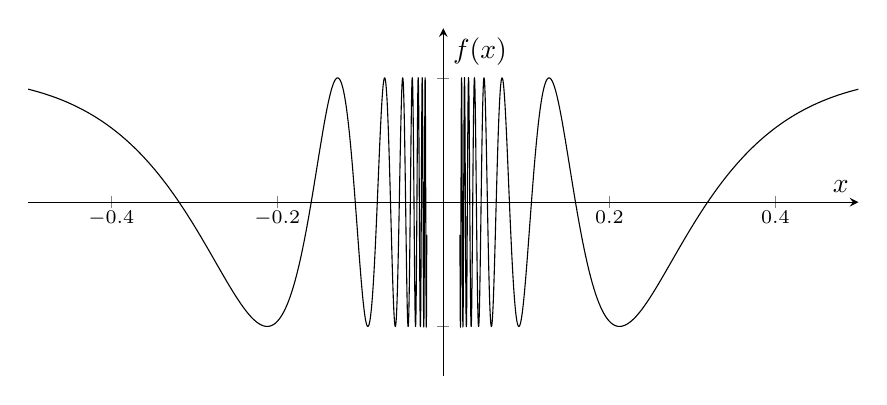
\begin{tikzpicture}
    \begin{axis}[
        width=\linewidth,
        height=6cm,
        axis lines=center,
        xlabel={$x$},
        ylabel={$f(x)$},
        ytick={-1,1},
        yticklabels={},
        xticklabel style = {
          font=\scriptsize,
          inner sep=1pt
        },
        xtick={-0.4,-0.2,0.2,0.4},
        xmin=-0.5, xmax=0.5,
        ymin=-1.4, ymax=1.4,
        samples=2500
      ]
      \addplot[black, domain=0.5:50] ({1/x}, {sin(deg(x))});
      \addplot[black, domain=0.5:50] ({-1/x}, {sin(deg(x))});
    \end{axis}
  \end{tikzpicture}
  \caption{$f(x)=\sin(1/x)$.}
  \label{fig:sin1x}
\end{figure}

This function oscillates wildly as $x \to 0$ and so does not approach any value at $x=0$. The intuition for this fact is that no matter how small we make an
interval containing $0$, we will always be able to choose a large enough natural number $n$, such that there is a point $a=\dfrac{2}{\pi(1+4n)}$ where $\sin{a}=1$, and
a point $b=\dfrac{2}{\pi(3+4n)}$ where $\sin{b}=-1$.

To prove that this limit does not exist we must first negate the definition of a limit. The function $f$ does \emph{not} approach $l$ near $a$ if
\[
  \exists \epsilon > 0 \text{ such that }, \forall \delta > 0,\ \exists x \text{ with } 0< |x-a| < \delta,\text{ and } |f(x)-l| \ge \epsilon.
\]
It is quite often the case that the easiest way to prove the nonexistence of a limit is by contradiction.

Assume for contradiction that $\lim_{x \to 0}\sin{1/x}=l$. Let $\epsilon=1/2$ and $\delta > 0$. Now choose a sufficiently large natural number $n$, such that
$a=\dfrac{2}{\pi(1+4n)}< \delta$. Then, there will also be the point $b=\dfrac{2}{\pi(3+4n)} < a < \delta$. Then,
\begin{alignat*}{2}
  |f(a)-l| & = |1-l|   &  & < \epsilon = \dfrac{1}{2} \\
  |f(b)-l| & = | -1-l| &  & < \epsilon = \dfrac{1}{2}
\end{alignat*}

By the triangle inequality
\[
  |1+1| = |(1-l)+(1+l)| \le |1-l| + |1+l| < \dfrac{1}{2} + \dfrac{1}{2} = 1 \implies 2 < 1
\]
Which is a contradiction. So our original assumption that the limit exists and equals $l$ must be wrong. \qed

\subsection{A slightly more complicated example.}
\[
  f(x) =
  \begin{cases}
    0            & x \text{ irrational, } 0 < x < 1                     \\
    \dfrac{1}{q} & x = \dfrac{p}{q} \text{ in lowest terms, } 0 < x < 1
  \end{cases}
\]
\begin{figure}[H]
  \centering
  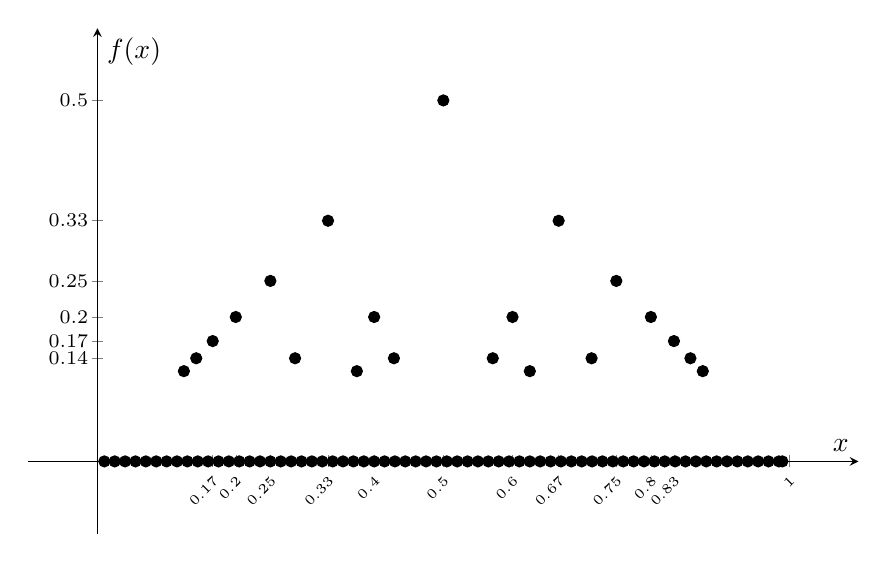
\begin{tikzpicture}
    \begin{axis}[
        width=\linewidth,
        height=8cm,
        axis lines=center,
        xlabel={$x$},
        ylabel={$f(x)$},
        ytick={1/7,1/6,1/5,1/4,1/3,1/2},
        xticklabel style = {
          font=\tiny,
          rotate=45,
          anchor=north east,
          inner sep=2pt
        },
        yticklabel style = {
          font=\scriptsize,
          inner sep=1pt
        },
        xtick={1/2,1/3,2/3,1/4,3/4,1/5,2/5,3/5,4/5,1/6,5/6,1},
        xmin=-0.1, xmax=1.1,
        ymin=-0.1, ymax=0.6,
        samples=100
      ]
      \addplot[only marks, mark=*, black] coordinates {
        (1/2,1/2)
        (1/3,1/3)
        (2/3,1/3)
        (1/4,1/4)
        (3/4,1/4)
        (1/5,1/5)
        (2/5,1/5)
        (3/5,1/5)
        (4/5,1/5)
        (1/6,1/6)
        (5/6,1/6)
        (1/7,1/7)
        (2/7,1/7)
        (3/7,1/7)
        (4/7,1/7)
        (5/7,1/7)
        (6/7,1/7)
        (1/8,1/8)
        (3/8,1/8)
        (5/8,1/8)
        (7/8,1/8)
      };
      \addplot[only marks, mark=*, black] coordinates {
        (0.01,0)
        (0.025,0)
        (0.04,0)
        (0.055,0)
        (0.07,0)
        (0.085,0)
        (0.1,0)
        (0.115,0)
        (0.13,0)
        (0.145,0)
        (0.16,0)
        (0.175,0)
        (0.19,0)
        (0.205,0)
        (0.22,0)
        (0.235,0)
        (0.25,0)
        (0.265,0)
        (0.28,0)
        (0.295,0)
        (0.31,0)
        (0.325,0)
        (0.34,0)
        (0.355,0)
        (0.37,0)
        (0.385,0)
        (0.4,0)
        (0.415,0)
        (0.43,0)
        (0.445,0)
        (0.46,0)
        (0.475,0)
        (0.49,0)
        (0.505,0)
        (0.52,0)
        (0.535,0)
        (0.55,0)
        (0.565,0)
        (0.58,0)
        (0.595,0)
        (0.61,0)
        (0.625,0)
        (0.64,0)
        (0.655,0)
        (0.67,0)
        (0.685,0)
        (0.7,0)
        (0.715,0)
        (0.73,0)
        (0.745,0)
        (0.76,0)
        (0.775,0)
        (0.79,0)
        (0.805,0)
        (0.82,0)
        (0.835,0)
        (0.85,0)
        (0.865,0)
        (0.88,0)
        (0.895,0)
        (0.91,0)
        (0.925,0)
        (0.94,0)
        (0.955,0)
        (0.97,0)
        (0.985,0)
        (0.99,0)
      };
    \end{axis}
  \end{tikzpicture}
  \caption{$f(x)$.}
  \label{fig:complicatedlimexample}
\end{figure}

Perhaps counterintuitively at the moment, this function approaches $0$ at $a$.
Recall the definition of a limit, the function $f$ \emph{approaches} $l$ at $a$ if for every
$\epsilon > 0, \ \exists \delta > 0, \text{ with }0< |x-a|<\delta, \text{ and } |f(x)-l|< \epsilon$.
We don't actually care what $f(a)$ is, since the difference between $x$ and $a$ will always be greater
than $0$, the value at $f(a)$ is irrelevant.

Perhaps an easier example of this idea is (\cref{fig:x2-1at0})
\[
  g(x) =
  \begin{cases}
    x^2 & x \ne 0 \\
    1   & x=0
  \end{cases}
\]
\begin{figure}[H]
  \centering
  \begin{tikzpicture}
    \begin{axis}[
        width=\linewidth,
        height=6cm,
        axis lines=center,
        xlabel={$x$},
        ylabel={$g(x)$},
        ticks=none,
        xmin=-2.5, xmax=2.5,
        ymin=-0.5, ymax=5,
      ]
      \addplot[black, thick, samples=100, domain=0.028:2] {(x^2)};
      \addplot[black, thick, samples=100, domain=-2:-0.028] {(x^2)};
      \addplot[only marks, mark=*, black] coordinates {
        (0,1)
      };
      \addplot[only marks, mark=o, fill=white, thick, black] coordinates {(0,0)};

    \end{axis}
  \end{tikzpicture}
  \caption{$g(x)=x^2$ except when $x=0$.}
  \label{fig:x2-1at0}
\end{figure}
Which still approaches $0$ as $x \to 0$. You can run through all the steps for the proof that $x^2$ approaches $a^2$ at $a$
above for this function if you need convincing.

Now for our proof that the $\lim_{x \to a}f(x)=0$ when $0<a<1$. Let $\epsilon > 0$ be given. Choose a sufficiently large
natural number $n$ such that $1/n < \epsilon$. The only numbers $x$ where $|f(x)-0|<\epsilon$ could be false are
\[
  \frac12,\ \frac13,\ \frac23,\ \frac14,\ \frac34,\ \frac15,\ \frac25,\ \mathellipsis,\ \frac{1}{n},\ \mathellipsis,\ \frac{n-1}{n}
\]
the set of which we can call $S$.

However many of these numbers there are, there are only finitely many, and so one of them is closest to $a$. That is,
$|p/q-a|$ is smallest for one specific $p/q \in S$. If $a$ is in $S$, then just consider all the elements of $S \ne a$.
If we chose $\delta$ to be this smallest distance then for all $x$ satisfying $0 < |x-a| < \delta$, $x$ is guaranteed not
to be in $S$, and therefore $|f(x)-0|<\epsilon$, which completes our proof. \qed

There is no need to give $\delta$ in terms of $\epsilon$, since there is nowhere in the definition
$\mathellipsis \forall \epsilon, \ \exists \delta \mathellipsis$ that says each $\epsilon$ needs a \emph{unique} $\delta$.

\section{Theorem 1-1}
\textbf{A function cannot approach two different limits near $a$}. If $\lim_{x \to a}f(x)=l$ and $\lim_{x \to a}f(x)=m$ then
$l=m$.

The proof of this assertion is a proof by contradiction very similar to the last example.

From the definition, for any $\epsilon > 0$ there is a $\delta_1$ such that if
\[
  0 < |x-a| < \delta_1 \text{ then } |f(x)-l|<\epsilon
\]
and a $\delta_2$ such that if
\[
  0 < |x-a| < \delta_2 \text{ then } |f(x)-m|<\epsilon
\]
So if we choose $\delta=\min(\delta_1,\delta_2)$ then if
\[
  0 < |x-a| < \delta \text{ then } |f(x)-l| < \epsilon \text{ and }|f(x)-m| < \epsilon
\]

Let $\epsilon = \dfrac{|l-m|}{2}$. Then for all $x$ satisfying $0 < |x-a| < \delta$
\begin{align*}
  |f(x)-l| & < \dfrac{|l-m|}{2} \\
  |f(x)-m| & < \dfrac{|l-m|}{2}
\end{align*}
From the triangle inequality
\begin{align*}
  |l-m| & = |(l-f(x))+(f(x)-m)|                 \\
  & \le |l-f(x)| + |f(x)-m|               \\
  & < \dfrac{|l-m|}{2} + \dfrac{|l-m|}{2} \\
  & = |l-m|
\end{align*}
which is a contradiction. \qed

\section{Theorem 1-2}
If $\lim_{x \to a}f(x)=l$ and $\lim_{x \to a}g(x)=m$ then
\begin{align*}
  \lim_{x \to a}(f+g)(x)       & =l+m       \\
  \lim_{x \to a}(f \cdot g)(x) & =l \cdot m
\end{align*}
In other words, the limit of sums is the sum of limits, and the limit of products is the product of limits.

Moreover, if $m \ne 0$
\[
  \lim_{x \to a} \left(\dfrac{1}{g}\right)(x) = \dfrac{1}{m}
\]
\chapter{Continuity}

\bibliographystyle{apalike}
\addcontentsline{toc}{chapter}{Bibliography}
\bibliography{refs}

\end{document}
